\chapter{Background}
\label{ch:related}

The acceleration of deep learning is an active topic of research and is
  cross-disciplinary by nature.
Much of this research happens around, inside of, or on top of
  dominant deep learning frameworks such as TensorFlow, PyTorch, and MxNet.
Research on these frameworks cuts across all abstraction levels and
  involves experts from machine learning, systems, architecture, and programming languages (PL).
Below we discuss various related topics necessary for understanding the work presented
  in this thesis, including the frameworks themselves, their programming model, compilation, execution and deployment.

\subsection{Deep Learning}

Deep learning (DL) has been used to achieve state-of-the-art results in
  applications ranging from computer vision to game
  playing to natural language processing.
Deep learning provides a collection of techniques for learning functions that are difficult
  to program directly.
A programmer solving a problem with DL performs three steps.
First, she specifies a parametric function (often called a \textit{model},
  \textit{neural network}, or simply \textit{network}) $F(\theta, x)$ of the function
  that computes the desired value.
She then \textit{trains} the model by applying an optimization algorithm to find a set of
  parameters $\theta$ that results in an acceptable approximation of the function on a
  collection of input-output pairs.
Finally, she uses her learned function to produce outputs for new inputs in
  a process called \textit{inference}.
While training and inference were once performed on the same machine,
  it is more common today to train models on a fleet of high-powered devices,
  since training is very computationally intensive.
The values learned from training can then be deployed for inference on less powerful systems,
  such as a single GPU, a mobile phone, or an FPGA.
This work is focused on helping a user wishing to utilize machine learning specify and optimize
  the neural networks they wish too with minimal fuss and maximal performance.

\section{Deep Learning Frameworks}

In the early days of deep learning, practitioners and researchers would program
  in general-purpose languages like Python utilizing
  scientific computing libraries like NumPy,
  which provide low-level \textit{operators} such as matrix multiplication.
In order to accelerate model execution,
    frameworks supporting accelerators such as GPU were introduced~\citep{theano} .
Early frameworks represented models as directed ``computation graphs'',
    where each node represents an operator,
    and each edge represents the flow of data from one operator to another.
Computation graphs provide a limited programming model,
    enabling straightforward mapping of operators onto GPUs.
Large technology companies,
    such as Google, Facebook, and Amazon,
    drive the development of frameworks,
    and consequently,
    each company has its own stack consisting
    of the core framework (TensorFlow~\citep{tensorflow}, PyTorch~\citep{pytorch}, MxNet~\citep{mxnet}),
    compilers(XLA~\citep{xla}, Glow~\citep{glow}, TVM~\citep{tvm_osdi18}),
    and hardware accelerators (TPU~\citep{tpuv1}, GraphCore, Inferentia~\citep{inferentia}).
Frameworks can be roughly categorized into those which support \textit{static} computation graphs
  and those which support \textit{dynamic} computation graphs.
Frameworks which use static graphs are said to be \textit{define-and-run} frameworks,
  whereas frameworks which use dynamic graphs are said to be \textit{define-by-run} frameworks.

\section{Define-And-Run Frameworks}

TensorFlow, Caffe~\citep{caffe}, and Theano~\citep{theano} are define-and-run frameworks.
Static graphs represent a whole-program,
  enabling optimization and simplified deployment,
  by removing the need for a host language like Python.
TensorFlow (TF) extends pure dataflow graphs with \textit{control edges}
      to emulate the functionality of \verb|if| and \verb|while|.
TF's representation captures many state-of-the-art models,
      provides support for heterogeneous hardware back-ends,
      and enables reverse-mode automatic differentiation~{\citep{ad_survey, tensorflow}}.
TF's encoding of control has limitations, as control-flow structures
    do not clearly map to familiar control-structures, instead using specialized
    encodings which make adapting traditional optimizations challenging.
Furthermore,
    unmodified TensorFlow does not support building models where the shape of
    the computation graph is dependent on the input,
    frustrating researchers who wish to experiment with complex models.
TensorFlow Fold addresses this \textit{particular} limitation~\citep{tensorflowfold}
    but offers no general and extensible solution.
% The encoding also requires \textit{ad hoc}, special-purpose operators such
%     as \verb|NextIteration| and the addition of special control edges to the graph.
The crux of the problem is the lack of generic mechanisms for users to
    define new control flow combinators (e.g., \verb|fold|) and data types.
% TensorFlow's programing model is relatively restricted and has led to a number
%     of solutions including TF Eager, AutoGraph, and JAX TODO CITE.
% Modifying frameworks in this manner is a considerable engineering effort
%     and does not scale.

\section{Define-By-Run Frameworks}
PyTorch~\citep{pytorch_ad}, Gluon~\citep{gluon}, Chainer~\citep{chainer_learningsys2015},
    and TensorFlow eager-mode~\citep{tf_eager} are define-by-run frameworks which
    attempt to address the challenges of previous work.
The approach popularized by PyTorch is to use a host language (e.g., Python)
    to eagerly execute operations while simultaneously building a computation graph
    as a side effect.
By using the full host language,
  its features may be used to provide a highly expressive programming model to users.
However, dynamic frameworks construct a graph \textit{per program trace} and must re-optimize when
    the graph topology changes, costing CPU cycles and incurring communication overhead between the host
    machine and accelerators.
Instead of just representing traces, \relay combines the advantages of both worlds by
    representing the whole program ahead of time,
    while supporting constructs like control flow, first-class functions, and data structures.

\section{Low-Level Tensor Compilers}
Low-level tensor compilers are focused on the production
    of high-performance operators which implement compute-intensive
    operations such as matrix multiplication or convolution.
There are a number of competing approaches,
    both from academic and commercial entities, such as
    TVM~\citep{tvm_osdi18}, Halide~\citep{halide}, Tensor Comprehensions(TC)~\citep{tensor_comprehensions},
    and Diesel~\citep{diesel}.
The most notable designs are either inspired by the
    compute-schedule split introduced by Halide
    and adapted by TVM, or the polyhedral framework,
    as used by TC and Diesel.
% Early frameworks relied heavily on manually optimized operator libraries for GPUs (e.g., cuBLAS and cuDNN).
Operator compilers perform code generation for sets of scalar loop nests,
    but only represent a restricted subset of a whole program, ignoring details such as
    memory allocation/management, data structures, closures, and arbitrary control flow.
\relay focuses on composing generic operators, and the surrounding program
    into an efficiently orchestrated DL program.

\section{Deep Learning Compilers}

DL frameworks have adopted compilers
    to tackle both performance and portability
    for existing applications, most notably
    XLA~\citep{xla}, Glow~\citep{glow}, nGraph~\citep{ngraph}, ONNC~\citep{onnc},
    PlaidML~\citep{plaidml}, and ModelCompiler.
These \textit{graph compilers} use computation graph IRs and provide
    lowering onto a variety of targets.
Often graph compilers only perform high-level optimizations
    and then offload to vendor-specific libraries.
% % TODO(this point is dangling)
% In particular,
%     XLA has advanced support for the TPU,
%     and is focused on lowering static loop nests into efficient kernels.

Due to their limited programming model, they
    provide the same functionality as \relay with
    a more limited language.
The most comparable points to \relay are recent
    developments in the TensorFlow and PyTorch
    ecosystems of MLIR and TorchScript, respectively.
Google introduced MLIR as a path forward for
    unifying its myriad of IRs.
Upon first examination MLIR might appear to be
    a replacement for XLA and related TF compiler
    efforts, but it is not that.
MLIR is shared infrastructure for constructing
    a set of interoperating IR ``dialects'' which
    can be used to construct compilers.
The MLIR project is working on IR dialects
    for TF's IR and a low-level polyhedral IR,
    but does not yet have an end-to-end solution for
    deep learning built upon MLIR, the insights in
    this paper can guide MLIR's dialect development.

TorchScript is a high-level Python-like IR developed as the first
    layer of PyTorch's JIT compiler.
PyTorch (since v1.0) can rewrite a subset of user programs into
    TorchScript, an idealized subset of Python.
TorchScript can then be executed by the TorchScript VM or JIT-compiled to a target platform.
TorchScript sits many layers above code generation and must accommodate
    the flexible semantics of Python, which rules out entire classes of static analysis.
In order to optimize away this dynamic behavior, TorchScript has
    a profiling JIT mode which identifies stable program traces
    during execution.
These stable static traces can then be optimized by lower-level
    compilers such as Glow or \relay to perform the last level of code generation.
Microsoft released ModelCompiler, a system for efficiently compiling RNNs defined
    in CNTK to CPU.
ModelCompiler uses Halide to represent low-level operations, but lacks
    the expressivity of the \relay IR and only demonstrates support for CPUs.
% \TQC{The discussion in this paragraph was a bit long given the less importance of this compiler,
%   consider remove everything except for
%   the paragraph about expressivitity.
%   I think we can even safely remove this paragraph
%   and fold it to citations to ngraph etc. mention lack of expressivity.
%   It is a workshop paper of LearningSys 18 workshop
%   \url{http://learningsys.org/nips18/assets/papers/30CameraReadySubmissionmodelcompiler_camera_ready_no_final_flag.pdf}
% }
% \todo{Suggestion from OOPSLA reviewer A: ``Accelerating recurrent neural networks through
% compiler techniques and quantization,'' Li-Wen Chang et al., Workshop on Systems for
% ML, NeurIPS 2018.}
% ModelCompiler similarly uses Halide to represent low-level operations,
%     which provides fusion and other standard optimizations.
% Their high-level IR is not clearly described but appears to lack arbitrary
%     control-flow, first-class functions, or datatypes.
% They employ quantization but do not demonstrate how/if it can be extended,
%     or if low-bit (< 8) quantization is supported.
% They have shown support for CPU execution but provide no
%     story for GPUs or accelerators.

\subsection{Programming Languages for Deep Learning}
\label{sec:pl_techniques_in_dl}

% TODO ADD tensor type sytems cites
In recent years, the design of new programming languages,
    or the augmentation of existing ones, has become
    a popular area of research.
New languages designed for machine learning and related
    tasks include Lantern~\citep{lantern}, Lift~\citep{lift_lang}, Flux.jl~\citep{fluxjl}
    AutoGraph~\citep{moldovan2018autograph}, Swift for TensorFlow~\citep{tf_swift},
    and JAX~\citep{jax}.
Lantern \citep{lantern} is the most related work to \relay as it can
    be used as a code generator.
Lantern is a deep learning DSL in Scala
    that uses lightweight modular staging (LMS) to lower code into C++ and CUDA.
Lantern's defining feature is the use of delimited continuations to perform
    automatic differentiation.
Delimited continuations provide an elegant algorithm for AD,
    only requiring local transforms, but incurs cost of
    heap allocated structures, and a less straightforward
    mapping to define-by-run frameworks.
Lantern solves this problem by using a CPS transform which
    complicated further optimization and code generation.
Lantern does not yet support hardware accelerators, and
    does not focus on full program optimizations.
The alternative approach is the augmentation of languages to support deep learning,
  the most notable being systems like AutoGraph, Flux.jl, Swift for TensorFlow,
  and JAX.
These systems are designed to be user-facing programming
    environments for deep learning and use a compiler IR
    to generate code.
For all intents and purposes \relay could be the IR in
    question, therefore  \relay complements these systems well by
    providing a more expressive IR to map computation onto.

    \section{Related Work}
\label{ch:related}

% 2. Related work including a discussion of how your proposed work either
% leverages that work (e.g., techniques you plan to adopt) or differs from it
% (e.g., novel contributions).  For your generals report, we recommend you
% focus primarily on your work on Beacon for high-level frontends, Relay for IR
% design, and type-supported optimizations for diverse backend support.

In this section we will focus on related work, specifically deep learning
frameworks, IRs and compilers, low-level tensor code generation DSLs,
prior work on deep learning and programming languages, dynamic neural
networks, and hardware acceleration for deep learning.

\subsection{Deep Learning Frameworks}

In the past few years deep learning has become an essential
  piece of technology to large companies which rely heavily
  on machine learning powered services.
Technology companies such as Facebook and Google have large development
  teams dedicated to developing tools to support deep learning research
  and development.
Google is developing an ML stack comprised of
  TensorFlow, XLA, TPU, and a host of satellite projects.
Facebook is developing an ML stack comprised of
  many projects including PyTorch,
  Glow~\citep{glow}, and Caffe2~\citep{pytorch_caffe2}.
Amazon Web Services has been developing a stack
  comprised of many projects including
  MxNet, TVM, and Inferentia.

In the early days of deep learning, users would program
  in general purpose languages like Python and utilize
  scientific computing libraries like NumPy,
  which provides low-level \textit{operators} such as matrix multiplication.
Operators, also called kernels,
  are dense linear algebra primitives like matrix multiplication,
  elementwise functions like \verb|tanh|, and complex,
  domain-specific operations like image convolution.
Operator execution dominates the execution time of a deep learning model: many
  operators are asymptotically slow and their input is large.
While a machine learning framework may be written as a library in a high-level language
  like Python or Swift, operators will typically be provided as opaque function calls to
  specialized implementations written in a lower-level language like C++.

To obtain better performance, researchers began utilizing specialized
  accelerators such as GPUs to accelerate the execution of models.
In order to accessibly provide acceleration to end-users
  researchers designed frameworks like Theano~\citep{theano}.
Frameworks such as Theano and Torch introduced a model of
  computation graphs, dataflow graphs composed of nodes of
    variables, and operations on data.
These computation graphs represent the AST of a small
  embedded DSL that could be easily compiled and deployed
  to accelerators like the GPU.
``Computation graphs'' provide a limited programming model,
    enabling efficient deployment.
Computation graphs have since been adopted as the fundamental building block of modern
    machine learning libraries.

Unfortunately computation graphs are an ad-hoc language engineered to solve
  the problems faced at the time, and do not begin to capture the full breadth
  of models that users would one day want to run.
For example,
  convolutional neural networks (CNNs),
  which are widely used in image processing and computer vision,
  generally utilize a fixed topology of layers
  with tensors of fixed dimension.
In contrast,
  recurrent neural networks (RNNs),
  which are widely used in natural language processing (NLP),
  require recursion, control flow, and
  operations over variable-sized data structures (e.g., lists).
The regular structure of CNNs facilitates
  optimizing compilation to
  common hardware accelerators (e.g., GPUs), but
  RNN-like models are still challenging to optimize.

One area in which deep learning has made significant advances since
  the introduction of early frameworks is natural language processing (NLP).
Reasoning about text requires context-sensitive analysis and data of
    non-fixed dimensions, unlike in many vision tasks.
 To allow for context-sensitive analysis, DL researchers have developed networks with persistent
  state, known as \textit{recurrent neural networks}  (RNNs).
Recurrent neural networks have found use not only in NLP, but also in speech recognition, music
  transcription, eSports, and other areas \citep{lstm, speech_recognition, OpenAI_dota}.
Unfortunately, since most machine learning frameworks rely on computation graphs,
  which cannot directly represent recursion, RNNs are usually finitely unrolled to a fixed depth.
This is acceptable if the depth can be determined statically and the loop unrolled
  ahead of time; however, if the depth depends on runtime values or complex control flow,
  unrolling must be performed dynamically.

There are two dominant designs for computation graph-based frameworks.
The first is the declarative design employed by TensorFlow.
Such designs extend pure data-flow with \textit{ad hoc} control operations
  to emulate the functionality of \verb|if| and \verb|while|.
This approach is called \textit{define-then-run} and employs \textit{static
computation graphs}.
A framework using a define-then-run representation has access to the entire
  graph before execution, providing more opportunities to optimize the program
  as well as simplifying deployment since the program can be executed
  without the host language.
However, the control flow structures are less expressive than those supported
  by the host language, frustrating researchers who wish to experiment with complex models.
For example, TensorFlow supports loops,
  but the elaborated graph has little resemblance to the input program, requiring optimization
  authors to reason about the elaborated form instead of familiar loops.
The encoding also requires \textit{ad hoc}, special purpose operators such
  as \verb|NextIteration| and the addition of special control-edges to the graph.
There are no generic mechanisms for users to define new control flow
  combinators (e.g., \verb|fold|) or data types.
TensorFlow's representation is sufficient for many state-of-the-art models,
  is easily ported to heterogeneous hardware back-ends,
  and allows for reverse-mode automatic differentiation~{\citep{ad_survey, tensorflow}}.

The second approach is used by PyTorch, where the host language (e.g. Python) dynamically
  constructs a computation graph.
This approach is called \textit{define-by-run} and employs \textit{dynamic computation graphs}.
An arbitrary host program executes dynamically, generating a computation graph as a by-product,
  allowing for use of all host language features.
However, by not encoding control constructs in its IR, a framework
  using define-by-run cannot reason about or optimize control flow structures.
Not only does this leave performance on the table, but it prevents deployment to certain
  edge devices, since they may have control flow or memory requirements that cannot be
  guaranteed by a fully dynamic control plane.

Dynamic frameworks such as  PyTorch~\citep{pytorch_ad},
    Gluon~\citep{gluon},
    Chainer~\citep{chainer_learningsys2015},
    and TensorFlow eager-mode~\citep{tf_eager} are attempts to alleviate the
    challenges of static graph representations
These dynamic frameworks must re-optimize and rebuild as graph topology changes, costing
    CPU cycles and incurring communication overhead between the host machine and accelerators.
Relay is designed to solve many of the challenges with existing work, as
  discussed in Section \ref{sec:past}.

There is work from frameworks on trying to balance tradeoffs, most of which has
  been realized using advanced compilers.
There are a large number of deep learning compilers being
  developed today but have relatively similar designs.
The Glow compiler~\citep{glow} provides a graph-based IR designed for lowering
  to hardware accelerators.
XLA~\citep{xla}, within Google's TensorFlow, supports lowering statically sized
  loops nests down to existing vendor provided libraries or generating customized
  code platforms such as the Google TPU.
Intel's nGraph provides a similar graph-based IR, focused on representing DAGs
  of operations.
A serious challenge of these frameworks is the focus on a single layer of the
  stack, and restricted semantics, these challenges introduce the lack of
  flexibility discussed in Section \ref{sec:intro}.

\section{Hardware Backends}

Even if a model can execute on
  a particular hardware device, developers
  often manually design model
  variants for each target platform
  to achieve the best performance.
If a programmer wants to experiment with a new hardware device,
  she must manually account for variations in hardware intrinsics, data
  types, and data layout.
This is only possible if the device is supported by her framework of choice.
Even with the addition of device-specific code,
  there is no guarantee performance will be acceptable, let alone optimal
  (or even that there will not be regression).
Many existing IRs also do not support data-dependent control flow.
  platform's intrinsics and design.

Engineers design these platform specific model variants
  through tedious experimentation and framework-specific tweaks
  to achieve acceptable performance~\citep{mobilenet}. % xnor_net, squeezenet}.
For example,
  engineers may need to \textit{quantize} models
  by manually reducing numerical precision for a particular platform,
  sacrificing some accuracy for better performance~\citep{xnornet}.
Manually tuning models requires
  that engineers learn the details of
  each platform's
  unique data types, intrinsics, and memory systems~\citep{fb_fp_hw, tpuv1, brainwave, nn_on_si}.

The landscape of specialized hardware
  accelerators is also rapidly growing~\citep{
    moreau2018vta, OpenTPU, tpuv1}.
Accelerators provide an attractive way to decrease
  the execution time, memory and power consumption of models, as well
  as enable deep learning in new contexts.
Many deployment targets, such as mobile phones, are a heterogenous system
  consisting of a CPU, GPU, and customized machine learning accelerator.
Automatically targeting accelerators requires sophisticated compilers which
  must perform a variety of optimizations and schedule computation across
  heterogenous devices.
Hardware vendors need software stacks, often extending a deep learning
  compiler with support for their devices in the form of operations,
  optimizations, and datatypes.
It is essential that frameworks can adapt to new hardware devices
  with minimal changes to applications.
Relay provides an extensible framework for hardware accelerators,
  and implements a backend for \vta an emerging hardware accelerator\citep{moreau2018vta}.
We demonstrate how we can use an expressive general-purpose deep learning IR, plus
  a few platform specific optimizations

\subsection{High Performance DSLs for Tensors}

My work is focused on the end-to-end compilation of deep learning, and for
  this reason we do not directly focus on the generation of efficient low-level code for
  tensor operations.
Instead my work is focused on optimizing programs which make use of low-level operations
  and optimizations around programs which combine them with higher-level abstractions,
  like closures and datatypes.
In particular \relay is designed as an extension to \tvm~\citep{tvm_osdi18},
  a tensor expression language used for specifying dense array
  operations, to support full models.
Previous work on the \tvm focused on producing efficient operators
  (dense linear algebra kernels), such as generalized matrix multiplication (GEMM) and convolutions.
In theory \relay could use other high performance DSLs such as Halide~\citep{halide},
    which \tvm derived its IR, and its split computation and schedule model.
\todo{HALIDE EXPAND HERE}
Tensor Comprehensions (TC) shares common goals with the \tvm framework, but achieves its goal
through different techniques, such as polyhedral compilation rather than algorithmic
schedules. TC could replace \tvm in \relay{}'s compilation.
\todo{TC EXPAND HERE}

\subsection{Programming Language based Deep Learning}

My work is not the first attempt to apply programming language
    techniques to machine learning or problems such automatic differentiation.
\todo{LANTERN EXPAND}
Lantern \citep{lantern} is a deep learning DSL in Scala
    that uses lightweight modular staging (LMS) to lower code into C++.
LMS takes a graph as input from the user and converts it to an AST
    representation, similar to \relay's graph mode.
LMS removes unnecessary abstractions.
Going one step further than Lantern,
    \relay supports accelerators.

\verb|Flux.jl| \citep{fluxjl} is a DL library written in Julia \citep{julia}, a numerical
computing language. Like \relay, \verb|Flux.jl| adds shapes to the type system; however, unlike \relay, it
uses a mixture of compile-time inference and runtime checks to enforce shape constraints
\citep{jlmlpl} and cannot perform platform-specific optimizations. Unlike \verb|Flux.jl|, which
tightly coupled with Julia, \relay is language agnostic and decouples frontend and IR
considerations.
\relay's features, such as type inference and deployment to multiple back-ends, can
    be easily reused by frameworks in arbitrary languages.

Additionally, previous work in higher-order differentiation from the PL community
has informed \relay's design.
In particular, we draw inspiration from various implementations of
automatic differentiation \citep{beautiful_diff, ad_survey, haskell_ad, toplas_reverse, wang_reverse, DLS, DDF},
with particular attention to techniques that can compute higher-order gradients of higher-order programs.
\verb|Zygote.jl| \citep{zygotejl}, like \relay, uses source code transformations to
    implement automatic differentiation.

% end related

\section{Related Work}
\label{sec:relwk}

Systems for machine learning is an active research area with a variety of techniques for ML inference engines which support dynamic features, cross-platform execution, and per-platform code generation. We discuss related work below.

% \hide{
% \begin{table}[tbp]
% \begin{tabular}{|c||c|c|c|}
% \hline
% Frameworks      & \makecell{Multi-platform \\ Portability}  & \makecell{Model \\ Dynamism} & Compilation \\ \hline
% TF/TF Fold      &             \xmark                     &         \cmark              &  \xmark     \\ \hline
% PyTorch         &             \xmark                     &         {\bf !}              &  \xmark     \\ \hline
% MXNet         &               \xmark                     &         \cmark              &  \xmark     \\ \hline
% DyNet           &             \xmark                     &         {\bf !}              &  \xmark     \\ \hline
% Cavs            &             \xmark                     &         \cmark              &  \xmark     \\ \hline
% Glow            &             \cmark                     &         \xmark              &  \cmark     \\ \hline
% TVM             &             \cmark                     &         \xmark              &  \cmark     \\ \hline
% XLA             &             \cmark                     &         \xmark              &  \cmark     \\ \hline
% Nimble         &             \cmark                     &         \cmark              &  \cmark     \\ \hline
% \end{tabular}
% \caption{Summary of popular machine learning systems, in terms of whether or not being easy to port to multiple platforms, performant for dynamic model inference ({\bf !} means supported but not efficient), and capable of compiling kernels.}
% \label{tab:ml_systems}
% \end{table}
% }

\noindent
{\bf Deep learning frameworks} As a framework, TensorFlow~\citep{tensorflow} supports dynamism via the addition of control flow primitives such as \emph{switch} and \emph{merge} in its graph representation~\citep{yu2018dynamic}. Similarly, MXNet~\citep{mxnet, mxnet-control} uses operators such as {\em foreach}, {\em cond}, and {\em while\_loop} to support control flow. The main drawback of this approach is requiring a runtime that uses an inefficient and complex control flow encoding such as TesorFlow, or a hybrid runtime such as MxNet which is inflexible for deploying to edge devices. As a separate effort, TensorFlow Fold~\citep{tensorflowfold} adds front-end syntactic sugar to TensorFlow for simplifying dynamic models via dynamic batching. Specifically, TensorFlow Fold conducts an analysis of the user's provided computation graphs and identifies dynamic operations that can be batched together. Once such operations are found, it transforms them into an intermediate representation (IR) that can be ingested by TensorFlow for evaluation. The nature of this approach can introduce large overhead as each path must be executed as a different sub-computation graph, as well as limiting further optimizaiton.

Dynet~\citep{neubig2017dynet} and PyTorch~\citep{pytorch} use host language features to dynamically (i.e., Python's control flow) to construct a dynamic model architecture. This allows a friendly and flexible programming model.
%as users can conveniently write code which appears no different then standard Python.
However, it requires the creation of new static data flow graph for each path through the program introducing control flow overhead, and limiting the scope of optimization to a single trace through the program, a trace which often only executed once~\citep{xu2018cavs}. These challenges were similarly faced by tracing-JIT based systems in the JIT compiler literature. JAX~\citep{jax2018github} also supports both control flow and dynamic features in its programming model, but is fundamentally limited by the ability for XLA, TensorFlow's deep learning compiler to optimize and compile dynamic code. To the best of our knowledge XLA still requires all loop nests to be static at code generation time.

%JANUS~\citep{jeong2019janus} optimizes the dynamic model execution in TensorFlow via speculative execution. It converts an imperative program that contains control flow defined in the host language (Python) into a symbolic data graph in TensorFlow for better performance. However, the conversion is incomplete due to dynamic typing, control flow, etc. Therefore, Janus falls back to imperative execution in the host environment when certain assumption breaks, which can lead to performance loss. In addition, JANUS shares the limitation in portability with the underlying framework.
Jeong et al.~\citep{jeong2018improving} and JANUS~\citep{jeong2019janus} both extend TensorFlow to improve the performance for dynamic models. Jeong et al.~\citep{jeong2018improving} introduces the recursive data structure in the programming model to replace the control flow primitives in the tree-like models. The solution is hard to generalize to other dynamic models though. JANUS~\citep{jeong2019janus} optimizes the dynamic model execution in TensorFlow via speculative execution. However, the conversion from imperative programs in Python to symbolic data graph in TensorFlow is incomplete due to dynamic typing, control flow, etc. Therefore, JANUS suffers the performance loss when it falls back to imperative execution. In addition, both work share the limitation in portability with the underlying framework.

%is an extension on top of TensorFlow to address the execution challenges led by dynamic models. It aimed to take the advantage of expressiveness provided by frameworks to represent dynamic models and the performance benefit of ahead of time optimization. JANUS takes the model defined in TF Eager and relies on speculative execution to remove control flow for speeding up the execution. It works well on certain models that could be executed speculatively but still suffers from performance loss on the other models that fail for speculative execution\yida{also mention it is limited by the framework?}.

Deep learning frameworks rely on third-party libraries to implement operators with different data shapes, namely, they achieve good performance for models with dynamic shapes on a specific hardware platform only if the corresponding high-performance third-party library is both used and supports an operation. Therefore, frameworks generally perform poorly on devices, such as ARM CPU, which are not in the first tier of device support such such as Google's TPU or Nvidia GPU in TensorFlow.

\noindent
{\bf Runtime systems} To address frameworks' challenges with dynamism, e.g. prohibitively high overhead in reconstruction of computation graphs and difficulties in batching together computations with similar input shapes recent works has proposed deep learning runtime systems~\citep{xu2018cavs, gao2018low}. These techniques exhibited effectiveness in improving the performance of dynamic models. However, these approaches suffer from a common limitation--they all heavily rely on the third party libraries, such as cuDNN~\citep{cudnn} and MKL-DNN~\citep{mkldnn}, raising concerns about portability. In addition, they usually only support a narrow subset of dynamic models on each platform.

\noindent
{\bf Deep learning compilers} Unlike the deep learning frameworks, Nimble is designed as an end-to-end deep learning compiler The existing deep learning compilers, including XLA~\citep{xla}, TVM~\citep{tvm_osdi18}, and Glow~\citep{glow}, offer a means to compile deep learning models to run on multiple hardware platforms, but only focus on static models and fail to support models with dynamism.
MLIR~\citep{lattner2020mlir} provides compiler infrastructure for deep learning workloads which allows developers to implement new dialects and combine them into a sing application. Its graph-level dialect has the support for dynamism, but has not yet produced work demonstrating how to achieve good performance in dynamic scenarios.
Nimble enables a deep learning compiler to support dynamism in an efficient and flexible way by adding a dynamic type system, a dynamic code generator, a VM-based runtime and a series of dynamic-specific optimizations.

Nimble's compilation and VM design is largely inspired by production compilers and VMs, such as LLVM~\citep{llvm}, GCC~\citep{gcc}, and JVM~\citep{jvm}. These generic solutions are able to easily handle dynamic behaviors, such as control flow and variable-length input arrays. However, the design of these compilers are heavily tailored to the optimization and execution profile of traditional programs. These programs manipulate small scalar values and consist of a large number of low level instructions. These VMs have a large number of instructions, which requires instruction execution and dispatch to be extremely efficient. Instead, deep learning compilers like Nimble manipulate primarily tensor values using a relatively small number of coarse-grained instructions, i.e. 16 instructions are sufficient for the Nimble VM. The execution hotspots of DL workloads are the compute-intensive operators (i.e. convolution) over large tensors. Thus, the micro-optimization of VM instruction dispatch is not essential to overall performance.

\vspace{-1.5em}

\section{Background}
\label{sec:background}

% TODO: Jared broadly suggested cutting this section. We do need to remove a lot of content just to be
% under the page limit, so we should determine what, if anything, here needs to be kept. For example,
% is a broad introduction to deep learning really something a reader would expect? We could set up
% the problem of expressiveness and deployment in the intro and focus on what other frameworks fall
% short on and what we do differently.

In this section, we provide a brief background on contemporary deep learning,
  popular deep learning frameworks, and state-of-the-art
  models being developed.

\subsection{Deep Learning}

Deep learning (DL) has been used to achieve state-of-the-art results in applications ranging from
computer vision to game playing to natural language processing. Deep learning provides a collection of
techniques for learning functions that are difficult to program directly.

For example, suppose one wants to construct a function $f(x)$ to extract building addresses from
images of a street. One approach to writing $f(x)$ explicitly might be to write programs to identify
regions of the image that contain information pertinent to addresses (like street names or house
numbers), partition those regions into individual characters, and identify each character.
One may then write a program that chains together many such modules into a working system.
It would require hundreds, if not thousands, of human-hours of work and dozens of heuristics to
write any of those programs by hand, and there is no guarantee it will perform well.
By contrast, deep learning has, with relatively little code, been
used to approximate this entire recognition task with a single model. The learned system
outperforms all hand-crafted solutions \citep{streetview}.

A programmer solving a problem with DL performs three steps. First, she specifies a parametric
function (often called a \textit{model}, \textit{neural network}, or simply \textit{network})
$F(\theta, x)$ of the function that computes the desired value. She then \textit{trains} the model
by applying an optimization algorithm to find a set of parameters $\theta$ that results in an
acceptable approximation of the function on a collection of input-output pairs. Finally, she uses
her learned function to produce outputs for new inputs in a process called \textit{inference}.

In practice, DL engineers write procedural programs that manipulate \textit{tensors},
  multi-dimensional arrays of numbers.
These restrictions allow DL practitioners to take advantage of
  statistics, linear algebra, and real analysis.
In order to search for an assignment of parameters that produces a good approximation, we must first
  define what a ``good'' approximation of $f$ is and then find an algorithm that optimizes this metric.
The quality of an approximation is typically defined in terms of some ground truth to
  compare against $F(\theta, x)$.
This ground truth is usually provided in the form of a
\textit{training set}, a set of input-output pairs that has either been manually collected or
  extracted from an existing data set.
The function that scores the output of a network with respect
  to a ground-truth label is called the \textit{loss function},
\[
  L \colon (\text{input}, \text{output}) \to \text{network} \to \mathbb{R}^{\ge 0},
\]
which typically takes in an input-output pair and network and produces a non-negative real
number.

One method to optimize the network is to take the gradient of the loss function composed with the
candidate network for some input-output pair. The gradient of a function points in the direction of
steepest change, so subtracting some proportion of the gradient from the current parameters reduces
the loss of the network. This process is known as \textit{stochastic gradient descent (SGD)}, and it
is the basis for many deep learning optimization algorithms used today.

More formally, training updates the model parameters using the following algorithm:
\[
  \theta_{i+1} := \theta_i - \varepsilon\nabla[L((\text{input}, \text{output})) \circ F]\Big|_{\theta_i}
\]
for some small, positive $\varepsilon$. This update cycle is repeated in training until
the error is acceptable. The final values of the parameters are then used for inference.

While training and inference were once performed on the same machine, it is more common today to
train models on high-powered devices such as a fleet of cloud machines or a custom GPU farm, since
training is very computationally intensive. The values learned from training can then be deployed
for inference on less powerful systems, such as a single GPU, a mobile phone, or an FPGA.

\subsection{Deep Learning Framework Design and Limitations}

Popular deep learning frameworks began with designs
  optimized for different tradeoffs between
  expressivity, performance, and portability.
In the early days of deep learning, users would program
  in general purpose languages like Python and utilize
  scientific computing libraries like NumPy,
  which provides low-level \textit{operators} such as matrix multiplication.
Operators, also called kernels, are dense linear algebra primitives like matrix multiplication,
  elementwise functions like \verb|tanh|,
  and complex, domain-specific operations like image convolution.
Operator execution dominates the execution time of a deep learning model: many
  operators are asymptotically slow and their input is often large.
While a machine learning framework may be written as a library in a high-level language
  like Python or Swift, operators will typically be provided as opaque function calls to
  specialized implementations written in a lower-level language like C++.

In order to obtain better performance, researchers began utilizing specialized accelerators.
To expose accelerators to end-users without needing to write in low-level languages,
such as CUDA, researchers designed frameworks like Theano~\citep{theano}.
These frameworks represent computations using dataflow graphs
  (treating mathematical operations on data as nodes)
  and compile these graphs to deploy to
  accelerators like the GPU.
``Computation graphs'' provide a limited programming model,
  enabling efficient deployment.
Computation graphs have since been adopted as the fundamental building block of modern
  machine learning libraries.

There are two dominant designs for computation graph-based frameworks.
The first is the declarative design employed by TensorFlow.
Such designs extend pure data-flow with \textit{ad hoc} control operations
  to emulate the functionality of \verb|if| and \verb|while|.
This approach is called \textit{define-then-run} and employs \textit{static
computation graphs}.
A framework using a define-then-run representation has access to the entire
  graph before execution, providing more opportunities to optimize the program
  as well as simplifying deployment since the program can be executed
  without the host language.
However, the control flow structures are less expressive than those supported
  by the host language, frustrating researchers who wish to experiment with complex models.
For example, TensorFlow supports loops,
  but the elaborated graph has little resemblance to the input program, requiring optimization
  authors to reason about the elaborated form instead of familiar loops.
The encoding also requires \textit{ad hoc}, special purpose operators such
  as \verb|NextIteration| and the addition of special control-edges to the graph.
There are no generic mechanisms for users to define new control flow
  combinators (e.g., \verb|fold|) or data types.

The second approach is used by PyTorch, where the host language (e.g. Python) dynamically
  constructs a computation graph.
This approach is called \textit{define-by-run} and employs \textit{dynamic computation graphs}.
An arbitrary host program executes dynamically, generating a computation graph as a by-product,
  allowing for use of all host language features.
However, by not encoding control constructs in its IR, a framework
  using define-by-run cannot reason about or optimize control flow structures.
Not only does this leave performance on the table, but it prevents deployment to certain
  edge devices, since they may have control flow or memory requirements that cannot be
  guaranteed by a fully dynamic control plane.

\subsection{Dynamic Neural Networks}

One area in which deep learning has made significant advances is
  natural language processing (NLP), such as finding keywords in a
  research paper, determining the sentiment of a tweet,
  or summarizing a news article.
Reasoning about text requires context-sensitive analysis and data of
  non-fixed dimensions, unlike in many vision tasks.
To allow for context-sensitive analysis, DL researchers have developed networks with persistent
state, known as \textit{recurrent neural networks}  (RNNs). Like the simple networks described
earlier, these networks have an input and an output; however, they take an additional input and
produce an additional output known as the \textit{hidden state}. Beginning with an initial hidden
state and a list of inputs (for example, characters from a source text), one can produce a
list of outputs (for example, a translation of the source text). %, as in Fig.~\ref{fig:rnn_graph}.
Recurrent neural networks have found use not only in NLP, but also in speech recognition, music
transcription, eSports, and other areas \citep{lstm, speech_recognition, OpenAI_dota}.

Unfortunately, since most machine learning frameworks rely on computation graphs,
  which cannot represent recursion, RNNs are usually finitely unrolled to a fixed depth.
This may be acceptable if the depth can be determined statically and the loop unrolled
  ahead of time; however, if the depth depends on runtime values or complex control flow,
  unrolling must be performed dynamically.
% Since the source language is usually an interpreted language like Python, this process incurs significant
% overhead. Even when unrolling can be computed ahead of time, it destroys information about
% the original program, which can no longer be used for ahead-of-time optimization.

\subsection{Hardware Backends}

If a programmer wants to experiment with a new hardware device,
  she must manually account for variations in hardware intrinsics, data
  types, and data layout.
This is only possible if the device is supported by her framework of choice.
Even with the addition of device-specific code,
  there is no guarantee performance will be acceptable, let alone optimal
  (or even that there will not be regression).
Many existing IRs also do not support data-dependent control flow.
If she cannot capture her model (e.g., an RNN) in the IR,
  she cannot deploy to hardware backends without requiring a host to drive
  execution.
In order to effectively use these devices,
  engineers often redesign the model from scratch to better match the target
  platform's intrinsics and design.

% \begin{figure}[!h]
%   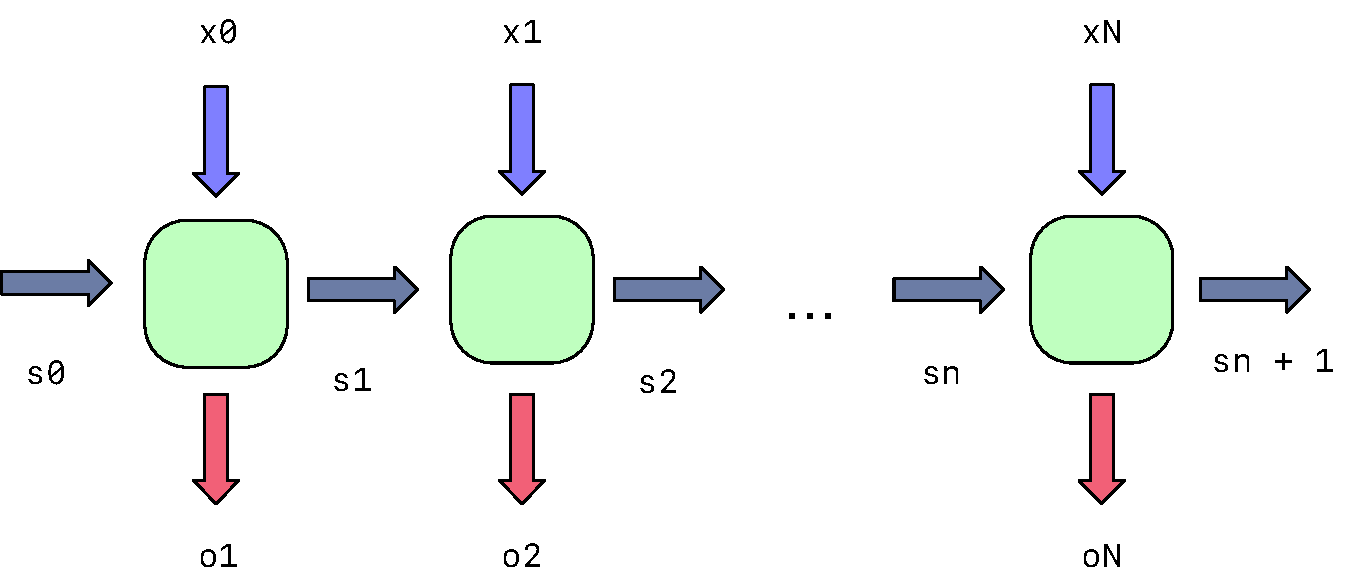
\includegraphics[width=0.9\columnwidth, height=5cm]{fig/rnn_graph}
%   \caption{
%     An RNN unrolled to time step $N$. The input arrows prefixed with $x$ are inputs,
%     the horizontal arrows prefixed $s$ are the hidden states, and the output arrows
%     are positional outputs of the model. For example each output would be a single
%     character of the names we generate in Section \ref{sec:overview}.}
%   \label{fig:rnn_graph}
% \end{figure}


% % For example,
% %   convolutional neural networks (CNNs),
% %   which are widely used in image processing and computer vision,
% %   generally utilize a fixed topology of layers
% %   with tensors of fixed dimension.
% % In contrast,
% %   recurrent neural networks (RNNs),
% %   which are widely used in natural language processing (NLP),
% %   require recursion, control flow, and
% %   operations over variable-sized data structures (e.g., lists).
% % The regular structure of CNNs facilitates
% %   optimizing compilation to
% %   common hardware accelerators (e.g., GPUs), but
% %   RNN-like models are still challenging to optimize.

% % INTEGRATE ME (DONE)

% % INTEGRATE ME PART 2
% % \subsection{Expressivity}
% % Most frameworks have employed a computation graph based IR.
% % These existing IRs are limited by their lack of flexibility as
% %   a programming language.
% % \todo{make this more crisp}
% % At first computation graphs appear to provide a compelling story for deployment to multiple devices.
% % Their emphasis on data flow makes it easy to port to new platforms, since one only has to think
% % about operators.

% % A limited programming model is both a strength and weakness,
% %   restricted semantics gives rise to efficient execution and
% %   straightforward portability.
% % Execution of a pure data-flow graph is well studied, and portability
% %   is determined by whether the platform has operator support.
% % Unfortunately the IR limits the set of programs that can be
% %   represented, recursive models such as RNNs and LSTMs
% %   can not be directly encoded and must be unrolled.
% % In order to grow the set of programs that can be represented,
% %   existing IRs have added numerous ad-hoc extensions.
% % For example, TensorFlow requires a complex
% %   encoding to support loops, and specialized containers such
% %   as TensorArray to support loop accumulation.
% % These extensions are enough to capture a set of
% %   useful models, but limit future extensibility.
% % For example there are no generic mechanisms for users
% %   to define new control flow combinators (e.g., \verb|fold|) or data types.
%   % ~\citep{
%   %   tf_fold, tangent, tf_eager, xla, glow, pytorch_caffe2}.
% % The deep learning community has seen multiple iterations
% %   of popular model architectures, and there
% %   is strong evidence user's needs will continue
% %   to evolve.

% \jmp{missing a so what here. imo it should be moved out of this section or cut entirely}
% New model architectures, such as the transformer, continue to
%   emerge, and the essential set of models, which demand
%   the best performance, continues to rapidly change.
% The transformer architecture itself is not yet two years
%   old, with multiple improvements published in just the past year.
% \todo{cites}
% A quickly evolving landscape requires frameworks,
%   and by extension their compilers, to adapt to emerging applications.

% % \subsection{Performance}
% \jmp{missing a so what for this paragraph}
% Even if a model can execute on
%   a particular hardware device, developers
%   often manually design model
%   variants for each target platform
%   to achieve the best performance.
% Engineers design these platform specific model variants
%   through tedious experimentation and framework-specific tweaks
%   to achieve acceptable performance~\citep{mobilenet, xnor_net, squeezenet}.
% For example,
%   engineers may need to \textit{quantize} models
%   by manually reducing numerical precision for a particular platform,
%   sacrificing some accuracy for better performance~\citep{xnor_net}.
% Manually tuning models requires
%   that engineers learn the details of
%   each platform's
%   unique data types, intrinsics, and memory systems~\citep{fb_fp_hw, tpuv1, brainwave, nn_on_si}.

% While a small number of transformations have been automated, they often lack flexibility and
% composibility. Consider quantization, the transformation that replaces floating point numbers with
% lower-precision fixed point numbers to trade model accuracy for speed and size. This transformation
% has been automated in TensorFlow with TensorFlow Lite~\citep{tflite}. To convert a TensorFlow model
% to a TensorFlow Lite model, a developer either runs quantization-aware training or converts a model
% directly to TensorFlow Lite. In either case, the bulk of the work is done by a translation from a
% TensorFlow computation graph to a TensorFlow Lite computation graph with 8-bit quantized operators.

% Although the TensorFlow Lite pass is straightforward, its design limits its extensibility. It does
% not allow for different or mixed precisions, let alone different quantization strategies.
% Furthermore, rather than using quantization like any other optimization, a developer must run a
% special converter to transform their TensorFlow computation graph into a quantized TensorFlow Lite
% computation graph, (presumably) precluding the use of TensorFlow optimizations on the quantized
% model.
% % TODO: cite https://www.tensorflow.org/lite/guide#tensorflow_lite_architecture and maybe some other
% % stuff, too

% TensorFlow Lite also rewrites much of the TensorFlow runtime system as well as bakes in 8-bit
% quantized operators. To gain full extensibility, operations would have to be written for every
% precision-platform pair.

% % \jmp{it's still not clear \textit{what} about existing frameworks prevents them from doing better}

% % A limited number of these transformations such as quantization have
%   % become automated, but are often inflexible and non-composable.
% % The rigidity of these passes are in contrast traditional
% %   compiler passes which are designed for composition.
% % Non-composable passes make it impossible for users to mix and
% %   match optimizations to suit their application needs, including
% %   integrating new optimizations.

% % \subsection{Portability}
% % \jmp{needs a topic sentence}
% % To further complicate matters the number of hardware platforms
% %   for deep learning is growing rapidly.
% % Beyond deploying machine learning in traditional services,
% %   developers may now train models in the
% %   cloud and deploy them to edge devices, such as mobile phones.
% % Many deployment targets, such as mobile phones, are a heterogenous system
% %   consisting of a CPU, GPU, and customized machine learning accelerator.
% % The number of specialized hardware
% %   accelerators available is rapidly growing~\citep{moreau2018vta, OpenTPU, tpuv1}.
% % Accelerators provide an attractive way to decrease
% %   the execution time, memory and power consumption of models while
% %   increasing the number of contexts deep learning can be deployed in.

% % Obtaining optimal performance from accelerators, requires
% %   mapping high-level computation to a device's limited
% %   instruction set.
% % Frameworks are often not designed for this use case \jmp{why not?} resulting in brittle
% %   software stack with support for a limited number of models.
% % Targeting accelerators requires sophisticated compilers which
% %   must perform a variety of optimizations and schedule computation across
% %   heterogenous devices.
% %   \todo{cite here, ask luis}
% % It is essential that frameworks can adapt to new hardware devices
% %   with minimal changes to applications.

Transforming Relay into code that executes efficiently on a variety of networks requires a series of transformations, and must interact with TVM and other layers below it.
